\section{Related Work}
\label{sec:related_works}
\subsection{fMRI-to-Image Reconstruction}
Recent methods for fMRI-to-image reconstruction leverage pretrained CLIP and SDXL models to predict image features. Notably, MindEye \cite{scotti2023reconstructingmindseyefmritoimage} predicts CLIP embeddings from fMRI and uses diffusion-based image generation to reconstruct seen images, while Brain-Diffuser \cite{ozcelik2023brain} combines visual representations with latent diffusion. MindEye2 further improves reconstruction through shared-subject training and predicts OpenCLIP ViT-bigG/14 representations \cite{schuhmann2022laionb, ilharco_gabriel_2021_5143773} for SDXL-based image generation. These approaches demonstrate the value of pretrained visual representations and generative models for fMRI-to-image reconstruction. However, most of these approaches operate on voxel- or region-of-interest (ROI)-based neural representations rather than cortical flatmaps. Our work instead investigates whether flatmap representations can provide a suitable input for modern vision architectures.

\subsection{fMRI Representations}
How fMRI activity is represented is a central consideration in developing generalizable neural representations. Traditional approaches reduce fMRI volumes with anatomical parcellations, producing compact feature vectors at the expense of spatial information. On the other hand, volumetric representations retain spatial structure but at a substantially greater computational cost. Recent fMRI foundation models have explored self-supervised learning to obtain general-purpose representations from large-scale datasets. For example, BrainLM \cite{Caro2023.09.12.557460} and BrainJEPA \cite{dong2024brainjepabraindynamicsfoundation}, among others, demonstrate the potential of pretrained models for downstream fMRI tasks. Notably, CortexMAE introduces cortical flatmaps as intermediate representations between parcellation and volumetric fMRI, converting cortical activity into 2D maps that can be processed by Vision Transformer architectures. Their results show that flatmaps preserve spatially structured information while also enabling patch-based processing. We build upon this representation by using a pretrained CortexMAE encoder to obtain spatially informed brain tokens for visual processing.

\subsection{Semantic and Low-Level Visual Features}
Faithful visual reconstruction benefits from both high-level semantic information and lower-level visual structure. CLIP and OpenCLIP provide semantic visual representations that have been widely adopted for image generation and brain decoding. At the same time, convolutional feature representations such as VGG \cite{simonyan2015deepconvolutionalnetworkslargescale} retain spatial information that may be lost in semantic embeddings. Recent brain decoding approaches have consequently explored multiple visual representations. MindEye and Brain-IT use semantic representations alongside lower-level visual features to improve image reconstruction. CortexDecoder follows this general pipeline by learning separate mappings from brain representations to OpenCLIP semantic tokens and VGG features, which are subsequently combined during image generation.

\begin{figure*}[!t]
\centering
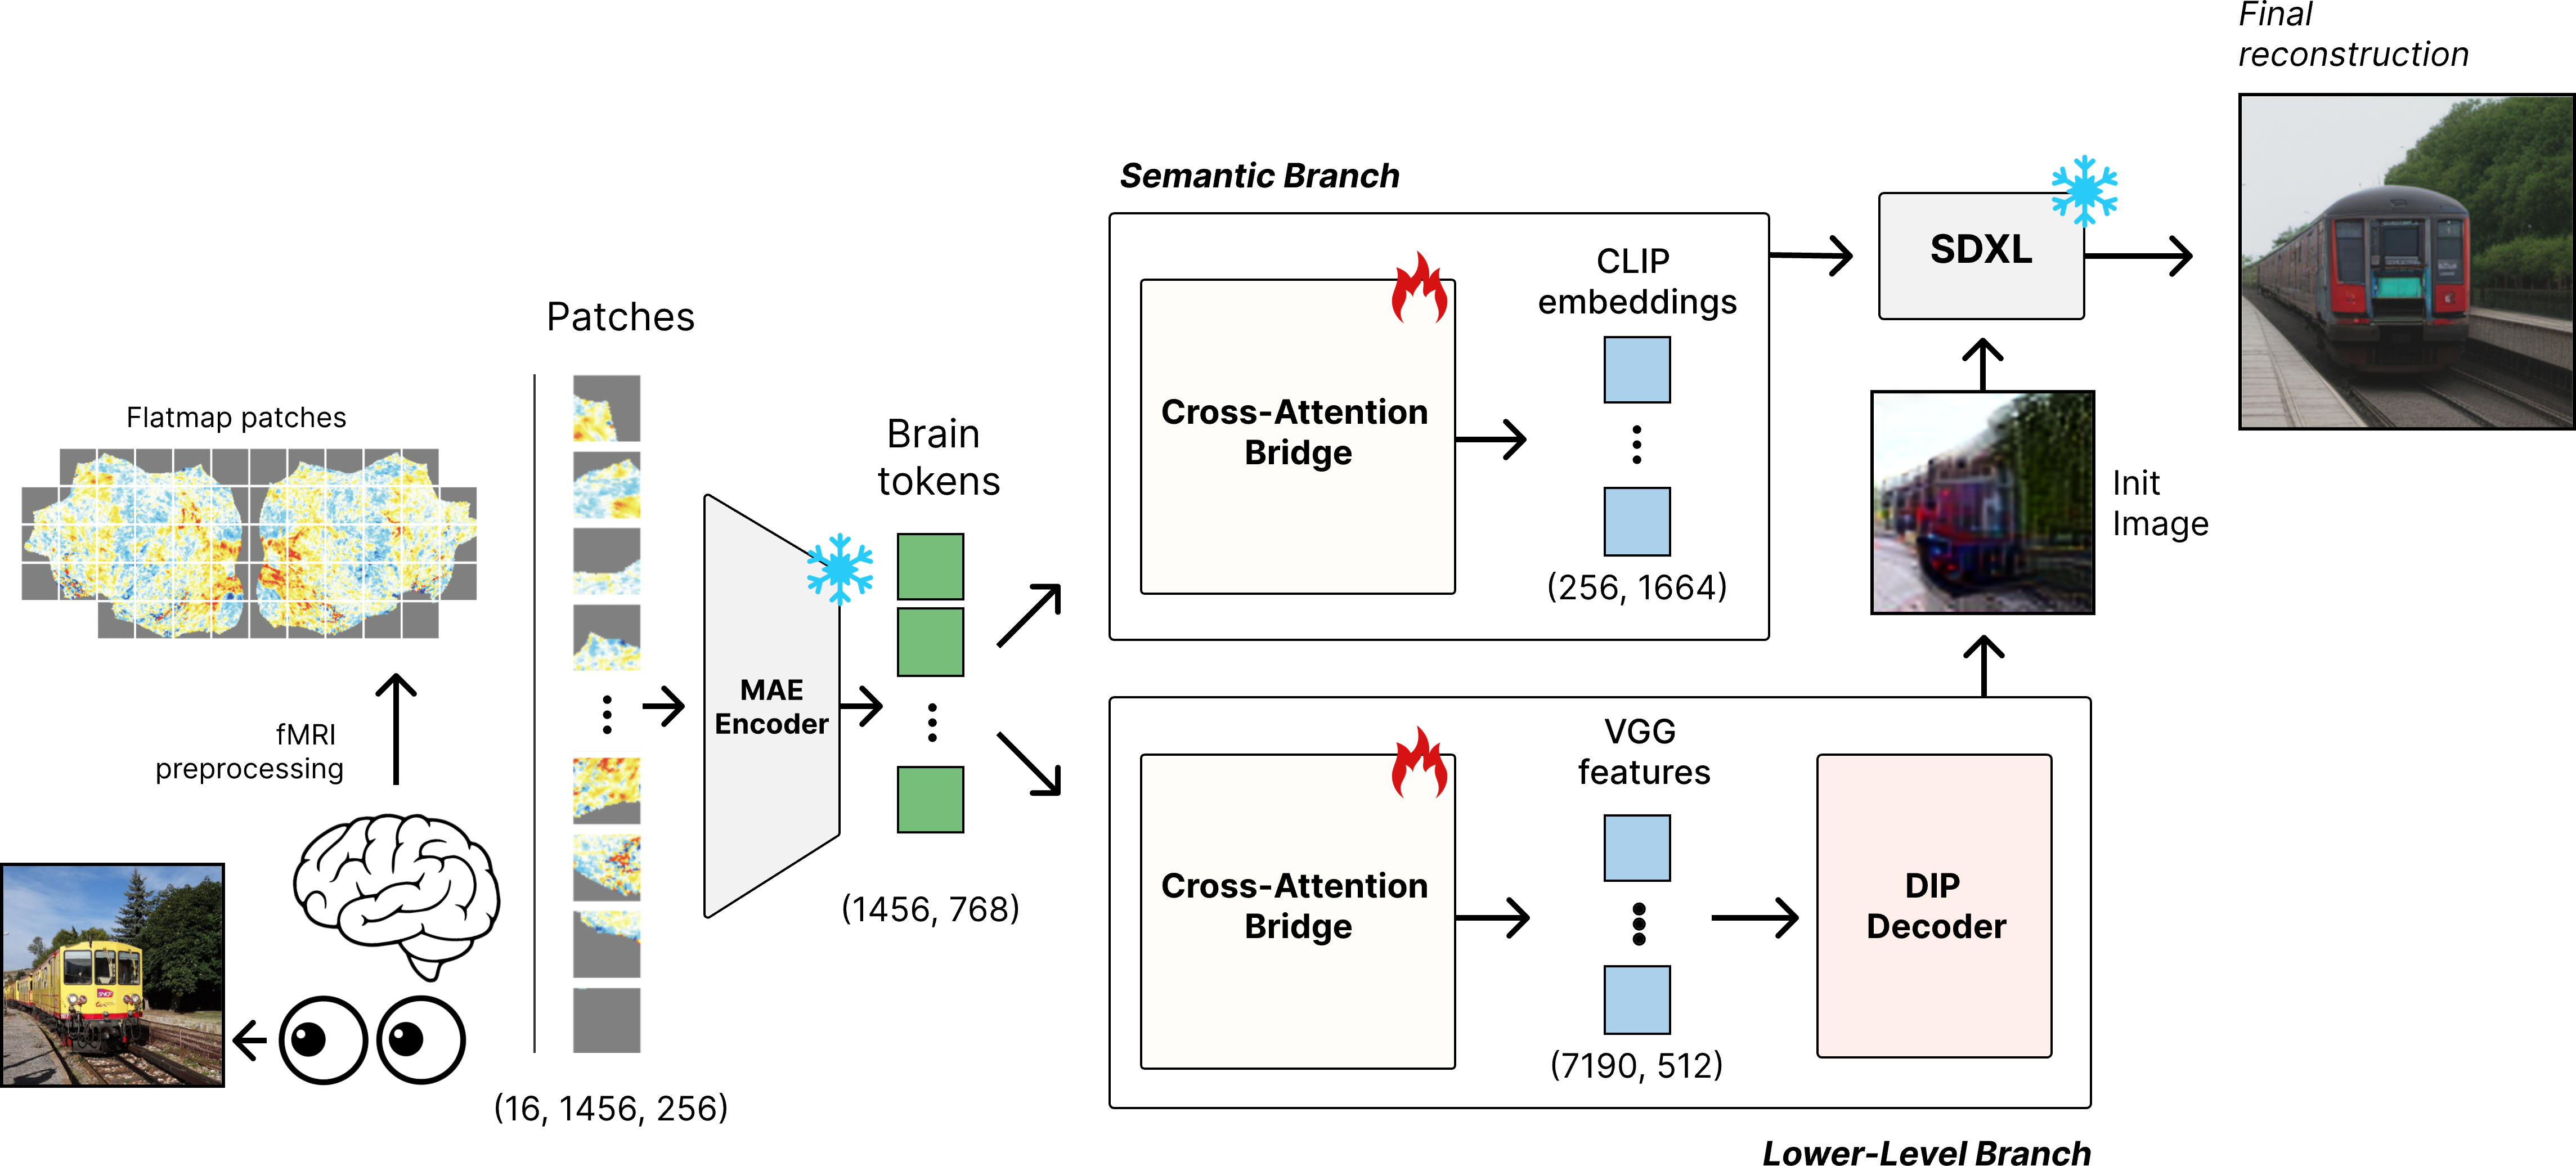
\includegraphics[width=0.75\textwidth]{images/model4.png}
\caption{CortexDecoder overview. A frozen CortexMAE encoder turns cortical flatmap patches into 1456 brain tokens. Two cross-attention bridges, the only trained components, predict OpenCLIP tokens (semantic) and VGG16-BN features (low-level). A DIP-inverted low-level image initializes SDXL-unCLIP, which is conditioned on the predicted OpenCLIP tokens to produce the final image. Images from COCO \cite{lin2015microsoftcococommonobjects} (CC BY 4.0).}
\label{fig:model_schematic}
\end{figure*}
